%%%%%%%%%%%%%%%%%%%%%%%%%%%%%%%%%%%%%%%%%
% University Assignment Title Page
% LaTeX Template
% Version 1.0 (27/12/12)
%
% This template has been downloaded from:
% http://www.LaTeXTemplates.com
%
% Original author:
% WikiBooks (http://en.wikibooks.org/wiki/LaTeX/Title_Creation)
%
% License:
% CC BY-NC-SA 3.0 (http://creativecommons.org/licenses/by-nc-sa/3.0/)
%
%
% ============Instellingen:============
%
%\documentclass[12pt]{article}
\documentclass[12pt,a4paper]{article}
\special{papersize=210mm,297mm}
\usepackage[top=2.5cm, bottom=3cm, left=2.5cm, right=2.5cm]{geometry}
%\usepackage[english]{babel}
\usepackage[dutch]{babel}
\selectlanguage{dutch}
\usepackage[utf8x]{inputenc}
%\usepackage{amsmath}
\usepackage{amsmath, amsthm, amssymb, amsfonts}
\usepackage{graphicx}
\usepackage{float}
\usepackage{caption}
\usepackage{subcaption}
\usepackage{wrapfig}
\usepackage{framed}
\usepackage{stfloats}
\usepackage{pdflscape}
% Maakt dat je landscape kan werken.
% Zie: https://www.ctan.org/pkg/pdflscape
\usepackage{csquotes}
\usepackage{multicol}
\setlength{\marginparwidth}{2cm}

\usepackage[colorinlistoftodos]{todonotes}
\usepackage{color}
% \colorbox{declared-color}{TO DO / ...}
% \textcolor{declared-color}{text}
%\usepackage{fontspec}
%\setmainfont{Calibri.ttf}

%\parskip = \baselineskip
% Bevel verplaatst na table of content.
% Vorig bevel: voeg een extra blanco lijn toe na elke paragraaf

\setlength{\parindent}{0em}
\usepackage{enumitem}

\captionsetup[figure]{name=Figuur}
% Om Nederlandse figuurnamen te hebben
\captionsetup[table]{name=Tabel}
%\captionsetup{font=footnotesize} toegevoegd om de bijschriften ook in een kleiner lettertype te hebben.
\captionsetup{font=footnotesize}

\addto\captionsenglish{% Replace "english" with the language you use
  \renewcommand{\contentsname}%
    {Inhoudstafel}%
}

%
% ============ BEGIN VAN HET DOCUMENT ============
%
%
\begin{document}

%Titelpagina....
% Titelpagina

\begin{titlepage}

\newcommand{\HRule}{\rule{\linewidth}{0.5mm}} % Defines a new command for the horizontal lines, change thickness here

\center % Center everything on the page
 
%----------------------------------------------------------------------------------------
%	HEADING SECTIONS
%----------------------------------------------------------------------------------------

\textsc{\LARGE KU Leuven}\\[1.5cm] % Name of your university/college


%----------------------------------------------------------------------------------------
%	TITLE SECTION
%----------------------------------------------------------------------------------------

\HRule \\[0.4cm]
{ \huge \bfseries xxxxxxxxxxxxxxxxxxxxxxxxxxxxxxxx}\\[0.4cm] % Title of your document
\HRule \\[1.5cm]
 
%----------------------------------------------------------------------------------------
%	AUTHOR SECTION
%----------------------------------------------------------------------------------------

\begin{minipage}{0.4\textwidth}
\begin{flushleft} \large
\emph{Student:}\\
Luc \textsc{Van Leuven} \\ % Your name
Jan \textsc{Peeters} % Your name



\end{flushleft}
\end{minipage}
~
\begin{minipage}{0.4\textwidth}
\begin{flushright} \large
\emph{Begeleiders:} \\
Patrick \textsc{Colleman} \\% Supervisor's Name
%Peter \textsc{Karsmakers} % second supervisor's Name


\end{flushright}
\end{minipage}\\[2cm]

% If you don't want a supervisor, uncomment the two lines below and remove the section above
%\Large \emph{Author:}\\
%John \textsc{Smith}\\[3cm] % Your name

%----------------------------------------------------------------------------------------
%	DATE SECTION
%----------------------------------------------------------------------------------------

{\large 1 mei 201x}\\[2cm] % Date, change the \today to a set date if you want to be precise

%----------------------------------------------------------------------------------------
%	LOGO SECTION
%----------------------------------------------------------------------------------------


\includegraphics[width=2.5in]{logokuleuven.png}\\[1cm] % Include a department/university logo - this % will require the graphicx package
 
%----------------------------------------------------------------------------------------

\vfill % Fill the rest of the page with whitespace

\end{titlepage}


\small
\tableofcontents
\newpage
\listoffigures
\newpage
\listoftables
% Volgend bevel staat pas hier, want anders staat er een blanco lijn na elke lijn in de inhoudstafel en de lijsten van figuren en tabellen:
\parskip = \baselineskip
\newpage
\Large
\textbf{Lijst van afkortingen}
\newline
\small
\begin{table}[ht]
% https://nl.wikibooks.org/wiki/LaTeX/Tabellen
\small
\begin{tabular}{ll} 
JSON        & JavaScript Object Notation \\
ifstream    & input file stream \\
Regex       & Regular Expressions \\
Abs.        & Absolute \\
Rel.        & Relative \\
VS          & Visual Studio \\
CPU         & Central Processing Unit \\
OC          & Overclocked \\
RAM         & Random Acces Memory \\
SSD         & Solid State Drive \\
VCS         & Version Control System \\
% AM &Amplitudemodulatie (Amplitude Modulation) \\
% DSN &Deep Space Network\\
% FM &Frequentiemodulatie (Frequency Modulation) \\
% NASA &National Aeronautics and Space Administration \\
\end{tabular}
\end{table}

\newpage

%\begin{multicols}{2}
\section{Inleiding}

\section{Teamwerk}
Één programma schrijven met meerdere programmeurs is niet simpel. Daarom gebruiken wij twee belangrijke tools. Met deze tools konden wij ons meer focussen op het programma zelf en minder op het oplossen van randproblemen.

\subsection{Git}
De eerste tool die wij gebruiken is Git.
Git is een \textit{Version Control System} (VCS) oftewel een versiebeheersysteem. De oorspronkelijke ontwikkelaar van git is Linus Torvalds in 2005.\cite{git:init} Ondertussen werken er al veel meer ontwikkelaars aan.

In een zogenoemde \textit{Git repository} worden alle verandering van code onthouden. Deze veranderingen slaagt men als programmeur op per nieuwe revisie. Deze revisies worden allemaal bijgehouden op chronologische volgorde. Zo kan men teruggaan naar een vorige revisie en deze vergelijken met de nieuwere revisie. Zo kan men de oorzaak van een fout sneller opsporen.

\subsection{Github}
De website \textit{www.github.com}, oftewel Github, is de tweede tool.
Deze website is een online platform voor versiebeheer via Git. Via Github kunnen programmeurs hun \textit{repository} online opslaan.\cite{git:hello_world} Zo kunnen zij altijd en overal aan hun code en deze ook snel delen met andere programmeurs.

\begin{figure}[ht]
    \centering
    
\includegraphics[width=0.4\textwidth]{illustraties/Octocat}
    \caption{Octocat, de mascotte van GitHub}
    \cite{git:github}
    \label{fig:octocat}
\end{figure}

\clearpage

\section{Boomstructuur}
\subsection{Tree-object}
\subsection{TreeNode-object}

\section{JSON}
De regressieboom wordt gegenereerd in python. Deze wordt dan gecodeerd en weggeschreven in JSON-formaat. Voor het inlezen van data in JSON-formaat bestaan al goede bibliotheken. Toch hebben we gekozen om dit zelf te programmeren. Wij waren namelijk ook intrinsiek gemotiveerd uit te zoeken hoe zo'n parser zou kunnen werken.

\begin{figure}[ht]
    \centering
    \lstinputlisting[language=JavaScript]{code/rules_d2.json}
    \caption{De boomstructuur in JSON-formaat}
    \label{fig:json_tree}
\end{figure}

Zoals te zien op Figuur \ref{fig:json_tree}, heeft elke node twee zogenoemde \textit{key-value pairs} of sleutel-waardeparen: \lstinline[language=JavaScript]{"key": "value"}. 
Deze zijn telkens gescheiden door komma's. Deze paren staan in een onbepaalde volgorde. Tijdens het lezen moeten we dus controleren waar elke sleutel voor staat.

\subsection{Sleutel: name}
In deze sleutel kunnen twee dingen staan. Als het een 
\subsection{Sleutel: children}

\section{Inladen van de structuur}

\section{Regex}
De beslissing of de prijs wordt opgeslagen in een string. Om deze data snel en foutloos uit deze string te halen gebruiken we regular expressions oftewel regex. Een zogenoemde regular expression is een reeks karakters die samen een patroon definiëren. Zo'n patroon wordt gebruikt om bepaalde dingen te zoeken, om speciefieke dingen te veranderen of om inputs te controleren.\cite{wiki:regex}

\subsection{Prijs}
\begin{lstlisting}[language=JavaScript]
{
    "name": "267 of Price",
    "children": null
}
\end{lstlisting}
\subsection{Beslissing}

\begin{lstlisting}[language=JavaScript]
{
    "name": "Model_B3 > 0.5",
    "children": [{...}, {...}]
}
\end{lstlisting}

\section{Testen}
In dit deel wordt getest hoe goed de pijsbepaling gebeurt bij bepaalde boomdieptes. Er wordt ook getest wat de invloed is van de boomdiepte op de tijd die het programma nodig heeft om de boom in te laden en om de prijs te bepalen. 

Om een zo accuraat mogelijk resultaat te bekomen, hebben we elke boom tienduizend, \(10^4\), keer ingeladen. Ook voor elke boom hebben we tien miljoen, \(10^7\), orgels geprijsd. De test duurde in totaal \(8.15613\) seconden. De resultaten zijn te zien in Tabel \ref{fig:test_result}.

\begin{table}[ht]
    \small
    \centering
    \begin{tabular}{|c|r|r|r|r|l|}
        \hline
        \bfseries Depth & \bfseries Load time & \bfseries Estimate time & \bfseries Total error & \bfseries Abs. error & \bfseries Rel. error\\
        \hline
        \csvreader[head to column names, late after line=\\]{data.csv}{}%
        {\depth & \load s & \est s & \total & \abs & \rel \%}
        \hline
    \end{tabular}
    \caption{Testresultaten}
    \label{tab:test_results}
\end{table}

De inlaadtijd van de boom is duidelijk afhankelijk van de boomdiepte. Bij een diepere boom zien we een duidelijke stijging in inlaadtijd. Met de grote-O-notatie is dit een complexiteit van $ O({2^n}) $. In dit geval is het geen worst case scenario omdat de boom niet overal vertakt tot beneden.

Bij het bepalen van de prijs zien we ook dat het langer duurt bij een diepere boom.

Bij het testen gebruiken we alleen orgels waarvan we de prijs kennen. Het programma maakt dan de schatting van de prijs. Deze prijs wordt dan vergeleken met echte prijs. Bij het nemen van de absolutewaarde van de fout en hier het gemmiddelde van te nemen over alle orgels krijgen we de absolute fout die te vinden is in de tabel. Het is heel dijdelijk dat deze fout kleiner wordt als de boom dieper wordt. Dit komt natuurlijk door dat er meer beslissing worden genomen en dus een betere prijsschating kan worden gedaan. Als we dan naar de procentuele fout gaan kijken, is deze bij een diepte van 5 heel klein. Daaruit kunnen we besluiten dat we bij een diepte van 5 een precise bepaling hebben van de pijs.

\begin{figure}[ht]
    \centering
    \begin{tikzpicture}
        \begin{axis}[
            width=0.7\textwidth,
            xlabel={Boom diepte },
            ylabel={Gem. ladingstijd (s)}]
            \addplot table [col sep=comma, x=depth , y=load] {data.csv};
        \end{axis}
    \end{tikzpicture}

    \begin{tikzpicture}
        \begin{axis}[
            width=0.7\textwidth,
            xlabel={Boom diepte },
            ylabel={Gem. uitvoertijd (s)}]
            \addplot table [ col sep=comma, x=depth, y=est] {data.csv};
        \end{axis}
    \end{tikzpicture}

    \caption{Grafieken Testresultaten}
    \label{fig:test_result}
\end{figure}

\subsection{Testomgeving}
In Tabel \ref{tab:pc-specs} staan de specificaties van de gebruikte computer. Van alle computers waarop we de test konden uitvoeren, was deze computer de snelste.

\begin{table}[ht]
    \centering
    \begin{tabular}{|l|l|}
        \hline
        \multicolumn{2}{|l|}{Software} \\
        \hline
        VS Build configuration  & Release x64 \\
        Besturingssysteem       & Windows 10 Pro 64-bit (10.0, Build 17763) \\
        \hline
        \hline
        \multicolumn{2}{|l|}{Hardware} \\
        \hline
        Processor               & Intel Core i7-7700K CPU @ 4.60 GHz OC (8 CPU's) \\
        Geheugen (RAM)          & 2x8.0 GB @ 2933 MHz \\
        Grafische kaart         & NVIDIA GeForce GTX 1080 Ti \\
        \hline
    \end{tabular}
    \caption{Specificaties van de gebruikte computer}
    \label{tab:pc-specs}
\end{table}


% We fixen de positie van deze figuur nog wel

%\section{Inleiding}

Communicatie met een ruimtetuig (voor bijvoorbeeld een Marsmissie) is cruciaal voor de goede werking van een verblijf in de ruimte om verschillende redenen. Enerzijds superviseert het controlecentrum op aarde de werking van de missie aan de hand van de resultaten van proeven, foto’s, meetwaarden, ... en anderzijds geeft het opdrachten door aan de bemanning en bestuurt het ruimtetuig.

De enige manier om te communiceren met een toestel in de ruimte zijn radiogolven.

Dit rapport gaat over een aantal principes om deze communicatie te realiseren. In een eerste deel gaat het over een beschrijving van het ‘Deep Space Network’ met het doel en de werking van de up- en downlink. In een tweede deel gaat het dieper in op fundamentelere onderwerpen zoals allereerst “Wat zijn radiogolven en hoe bevatten deze de informatie?”, vervolgens op “Hoe werken schotelantennes?” om te eindigen met “Waarom is communicatie met ruimtetuigen op grote afstand moeilijk?”.

\section{Communicatie met een ruimtemissie}

\subsection{Wat is het 'Deep Space Network'?}

Het ‘Deep Space Network’ (DSN), dat sinds 1958 als een onderdeel van NASA (National Aeronautics and Space Administration) bestaat, is een internationaal netwerk dat door middel van drie gigantische antennes op de aarde communicatie mogelijk maakt met satellieten of ruimtetuigen \cite{martin}. Het eerste deep-space communicatiecentrum is te vinden in de Mojave-woestijn in Californië nabij Goldstone, een tweede nabij Madrid in Spanje en een derde in Canberra, Australië. Door deze geografische spreiding, telkens ongeveer 120° verder op de aardbol, is steeds communicatie mogelijk met om het even waar in de ruimte \cite{christiaens}. 

\subsection{Wat is de uplink en de downlink bij een 'Deep Space Network'?}

De uplink is het verzenden van informatie vanop aarde naar een ruimtetuig. De uplink doet een upload. De downlink gaat in de andere richting: van een ruimtetuig naar de aarde. Deze doet een download. De vertraging is de tijd die verstrijkt tussen het verzenden en ontvangen van een signaal. Radiogolven zijn, net zoals licht, elektromagnetische golven. De voortplantingssnelheid is voor radiogolven 3.108 meter per seconde in lucht of het luchtledige. Dit lijkt snel, maar is eigenlijk (relatief) traag wegens de enorme te overbruggen afstanden \cite{updown}. Deze afstand is bijvoorbeeld gemiddeld 384 450 km tot de maan \cite{maan} en 230 000 000 km tot Mars \cite{mars}.

\subsection{Wat zijn radiogolven en hoe bevatten deze informatie?}

Elektromagnetische golven zijn, op basis van hun frequentie of golflengte, onder te verdelen in radiogolven, microgolven, lichtstralen, röntgenstralen, gammastraling, … \cite{radiowaves}, zoals te zien in figuur \ref{fig:EMS} op bladzijde \pageref{fig:EMS}.

\begin{figure}[ht]
  \centering
  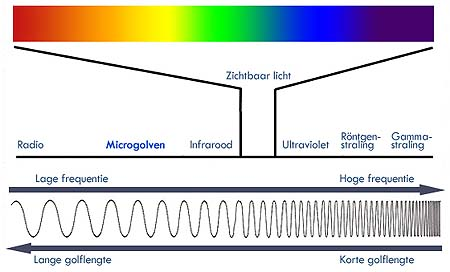
\includegraphics[width=0.5\textwidth]{voorbeeld_figuren/spectrum_straling}
  \caption{Elektromagnetische straling.} 
  \cite{energiezonnepanelen} %Als je deze cite in de caption plaatst, komt de referentie ook in de lijst van figuren voor en is de volgorde niet juist.
  \label{fig:EMS}
\end{figure}

De frequentie f van radiogolven is het aantal keer per seconde dat het signaal maximaal wordt. De eenheid van frequentie is Hz (Hertz). De golflengte is de afstand tussen één maximum en het volgende maximum van het signaal. De elektrische en magnetische component en voortplantingsrichting zijn te zien in figuur \ref{fig:golf} op bladzijde \pageref{fig:golf}.

\begin{figure}[ht]
  \centering
  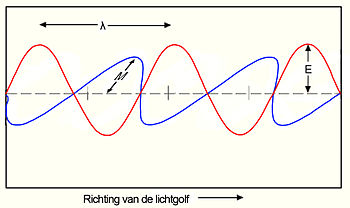
\includegraphics[width=0.5\textwidth]{voorbeeld_figuren/elektromagnetische_golf}
  \caption{Voortplanting elektromagnetische golf.} 
  \cite{elektromagnetischestraling}
  \label{fig:golf}
\end{figure}

Een zeer belangrijk verband tussen de frequentie f en de golflengte $\lambda$ is: $v = f\lambda$, met v de voortplantingssnelheid van de golf \cite{elektromagnetischestraling}. Bij een grotere golflengte zijn de golven immers breder en duurt het dus langer eer een volledige golf ergens voorbij komt (lagere frequentie). Deze tijd is de periode T. Er geldt: $T = \frac{1}{f}$. De golflengte van zichtbaar licht is (veel) kleiner dan van radiogolven: ordegrootte $10^{-6}$ meter. 

Radiogolven voor radio en TV hebben dan weer een grotere golflengte dan radiogolven voor communicatie in de ruimte. Bij deze laatste  is de golflengte zeer klein: ongeveer één centimeter. 

\begin{figure}[ht]
  \centering
  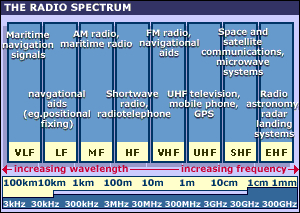
\includegraphics[width=0.5\textwidth]{voorbeeld_figuren/radiospectrum}
  \caption{Radiospectrum.} 
  \cite{wavelengths}
  \label{fig:radiospectrum}
\end{figure}

Een radiogolf voldoet aan de uitdrukking: 
\begin{equation*} %eventueel \label{} bijvoegen om te kunnen refereren.
v = A\sin(\omega t+\phi)
\end{equation*}	%equation zonder * geeft een nummer bij de uitdrukking. Dit is nodig als je naar deze formule wil refereren. 
Dit impliceert dat een golf informatie kan bevatten door ofwel de amplitude A ofwel de hoek $(\omega t+\phi)$ ofwel eventueel een combinatie van amplitude en hoek te veranderen. Bij amplitudemodulatie (AM) bevat de amplitude de informatie en bij frequentiemodulatie (FM) is dat $\omega$ \cite{radiowaves1}.  Hierbij is $\omega = 2\pi f$. Een variante op frequentiemodulatie is fasemodulatie (PM). Bij fasemodulatie is de fase een functie van het door te sturen signaal.

\subsubsection{Amplitudemodulatie}

Bij amplitudemodulatie \cite{kennedy} (AM) is de golfvorm het resultaat van een hoogfrequent signaal, de draaggolf met een vaste frequentie, waarvan de amplitude veranderlijk is naargelang de door te zenden informatie. Een positief (audio)signaal levert een iets hogere draaggolfamplitude, een negatief signaal levert een iets lagere draaggolfamplitude. Wiskundig is de amplitude van de draaggolf gelijk aan de som van een constant signaal (gelijkspanning) met het door te zenden signaal. De mate waarin de draaggolf het bronsignaal volgt, heet de modulatiediepte, uitgedrukt in procenten van de ongemoduleerde draaggolf. Deze is steeds kleiner dan 1. Figuur \ref{fig:AM} op bladzijde \pageref{fig:AM} toont een informatiesignaal, de ongemoduleerde draaggolf (carrier in het Engels) en ten slotte het resulterend signaal.

\begin{figure}[ht]
  \centering
  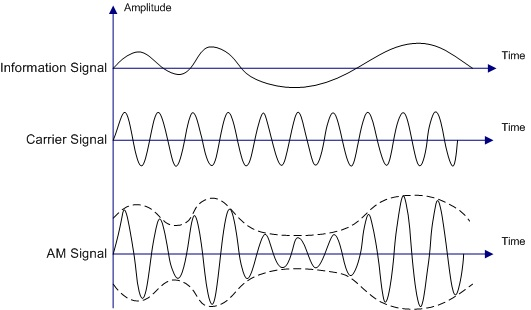
\includegraphics[width=0.5\textwidth]{voorbeeld_figuren/AM}
  \caption{AM modulatie.} 
  \cite{AM}
  \label{fig:AM}
\end{figure}

\subsubsection{Frequentiemodulatie} 

Bij frequentiemodulatie \cite{kennedy} (FM) is de bekomen golfvorm opnieuw het resultaat van een hoogfrequent signaal, de draaggolf, maar waarbij nu de amplitude constant is en de frequentie veranderlijk naargelang de door te zenden informatie. Hoe hoger de amplitude van het door te zenden signaal, hoe hoger de frequentie van de aangepaste draaggolf. Frequentiemodulatie is minder gevoelig aan ruis dan amplitudemodulatie. Daar staat wel tegenover dat een FM-signaal bij een gegeven bronsignaal in het algemeen, afhankelijk van de modulatie-index, veel meer bandbreedte nodig heeft dan een AM-signaal. Figuur \ref{fig:FM} op bladzijde \pageref{fig:FM} toont een informatiesignaal, de ongemoduleerde draaggolf (carrier in het Engels) en ten slotte het resulterend signaal (de gemoduleerde draaggolf).

\begin{figure}[ht]
  \centering
  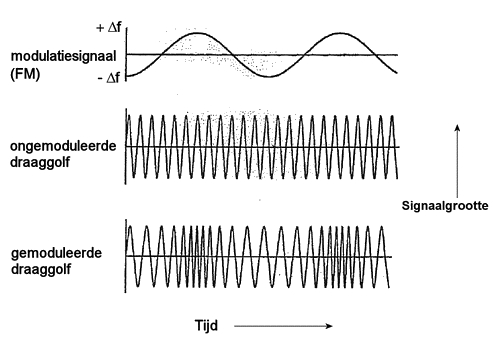
\includegraphics[width=0.5\textwidth]{voorbeeld_figuren/FMwit}
  \caption{FM modulatie.} 
  \cite{FM}
  \label{fig:FM}
\end{figure}


\subsection{Hoe werken schotelantennes?}

Elk type antenne heeft zijn toepassingsgebied. Voor communicatie met een ruimtetuig, zijn alleen schotelantennes bruikbaar \cite{kennedy}. De reden hiervoor is dat alleen schotelantennes hun energie in één welbepaalde enge bundel kunnen verzenden.

\begin{figure}[ht]
  \centering
  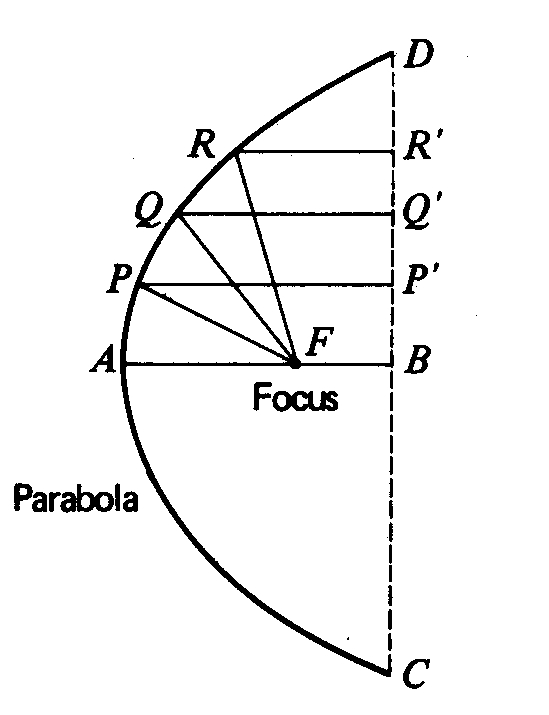
\includegraphics[width=0.3\textwidth]{voorbeeld_figuren/paraboolantenne_doorsnede}
  \caption{Doorsnede van een paraboolantenne.} 
  \cite{kennedy}
  \label{fig:parabool}
\end{figure}

Schotelantennes hebben een parabolische vorm, zoals te zien in figuur \ref{fig:parabool} op bladzijde \pageref{fig:parabool}. Een eigenschap van deze vorm is dat alle signaalenergie die erop invalt, wordt geconcentreerd in het brandpunt (focus) en omgekeerd dat alle energie die vertrekt vanuit het brandpunt naar de parabool, verder reist in een zeer gericht signaal. 

Kenmerkend voor schotelantennes is dat ze werken bij hoge frequenties en bijgevolg kleine golflengten.

Een antenne heeft als doel zoveel mogelijk het signaal in één richting te sturen. Dit lukt beter naarmate de golflengte kleiner en de antenne groter is. Communicatie in de ruimte vereist bijgevolg kleine golflengten en dus hoge frequenties. De antennes voor het Deep Space Network zijn bovendien zeer groot!

\subsection{Waarom is communicatie met ruimtetuigen op grote afstand moeilijker?}

De oppervlakte van een bol is gelijk aan $4\pi r^{2}$. Het ontvangen signaal op een bepaalde afstand r van de antenne is bijgevolg omgekeerd evenredig met $r^{2}$ of dus evenredig met $r^{-2}$. Wanneer de afstand dus verdubbelt, verkleint het vermogen van het signaal al vier keer! 

In het geval van communicatie met een ruimtetuig is de afstand zeer groot. Het ontvangen signaal is bijgevolg zeer klein en dus moet de schotelantenne zeer groot zijn om toch maar voldoende invallend vermogen te kunnen verzamelen in het brandpunt \cite{radiocontact}. Een voorbeeld hiervan is figuur \ref{fig:effelsberg} op bladzijde \pageref{fig:effelsberg}.

\begin{figure}[ht]
  \centering
  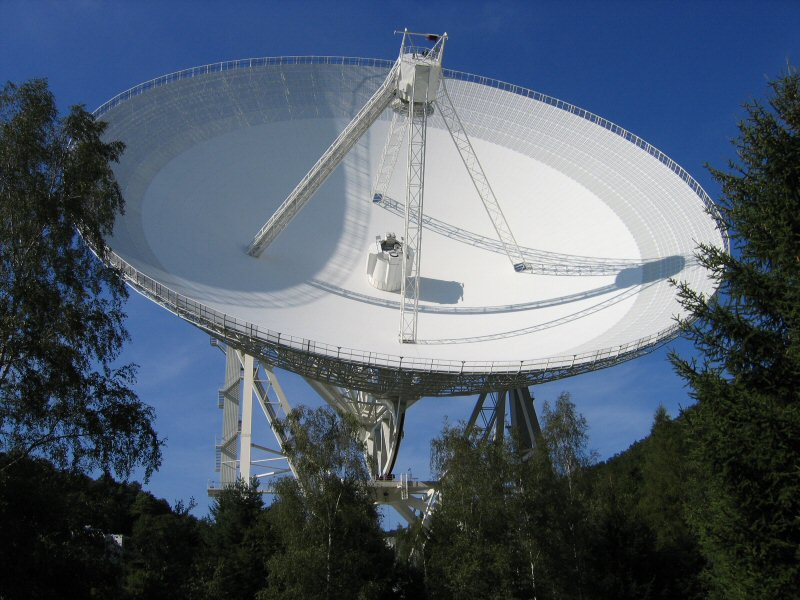
\includegraphics[width=0.6\textwidth]{voorbeeld_figuren/paraboolantenne}
  \caption{Effelsberg telescoop.} 
  \cite{effelsberg}
  \label{fig:effelsberg}
\end{figure}

\section{Geplande ruimtevluchten}

Een overzicht van toekomstige ruimtemissies naar de maan kan je vinden in tabel \ref{tab:missies} op bladzijde \pageref{tab:missies}.

\begin{table}[ht]
\centering
\small
\begin{tabular}{cc|c} %De | duidt aan waar je een verticale lijn in de tabel wil.
Land &Jaar &Missie \\ \hline
India &2018 &Chandrayaan-2 \\ 
Verenigde Staten &2018 &Lunar Flashlight \\ 
Verenigde Staten &2018 &Lunar Ice Cube \\ 
Japan &2019 &SLIM \\
Zuid-Korea &2020 &Moon orbiter \\ 
Verenigd Koninkrijk &2024 &Lunar Mission One \\
\end{tabular}
\caption{Land, jaartal en naam van enkele toekomstige missies.}
\cite{missies}
\label{tab:missies}
\end{table}

\section{Besluit}

Communicatie met een missie naar Mars is zeker mogelijk dankzij de zeer grote schotelantennes van het ‘Deep Space Network’. Deze antennes kunnen permanent voldoende sterke signalen uit de ruimte ontvangen of naar de ruimte versturen dankzij hun grote afmetingen, hun geografische spreiding en de gebruikte frequenties. Amplitudemodulatie of frequentiemodulatie zijn bruikbare technieken om de signalen uit te zenden of te ontvangen.
%\end{multicols}

\scriptsize
\newpage
\begin{flushleft}
\bibliographystyle{IEEEtran}
\bibliography{bronnen} %Je mag deze file een andere naam geven, maar de extensie moet 'bib' zijn.
\end{flushleft}

\end{document}
